% !TeX program = lualatex
% Gemini theme
% See: https://rev.cs.uchicago.edu/k4rtik/gemini-uccs
% A fork of https://github.com/anishathalye/gemini

\documentclass[final,10pt]{beamer}

% ====================
% Packages
% ====================

\usepackage[T1]{fontenc}
\usepackage{lmodern}
\usepackage[size=custom,width=72,height=48,scale=1.0]{beamerposter}
\usetheme{gemini}
\usecolortheme{uchicago}
\usepackage{graphicx}
\usepackage{booktabs}
\usepackage{tikz}
\usepackage{pgfplots}
\pgfplotsset{compat=1.16} %1.17
\usepackage{subcaption}

% ====================
% Lengths
% ====================

% If you have N columns, choose \sepwidth and \colwidth such that
% (N+1)*\sepwidth + N*\colwidth = \paperwidth
\newlength{\sepwidth}
\newlength{\colwidth}
\setlength{\sepwidth}{0.025\paperwidth}
\setlength{\colwidth}{0.3\paperwidth}
\usepackage{algorithmicx}
\usepackage{algpseudocode}
\usepackage{algorithm}
\usepackage{eqparbox}
\renewcommand\algorithmiccomment[1]{%
	\hfill\#\ \eqparbox{COMMENT}{#1}%
}
\newcommand\LongComment[1]{%
	\hfill\#\ \begin{minipage}[t]{\eqboxwidth{COMMENT}}#1\strut\end{minipage}%
}
\algnewcommand{\LeftComment}[1]{\Statex \(\triangleright\) #1}

\newcommand{\separatorcolumn}{\begin{column}{\sepwidth}\end{column}}

% ====================
% Title
% ====================

\title{An Adversarial Malware Evasion Attack Using Machine Translation}

\author{\textbf{Luke Kurlandski}, Yin Pan, Matthew Wright}

\institute[shortinst]{Rochester Institutute of Technology Department of Computing Security} 

% ====================
% Footer (optional)
% ====================

%\footercontent{
 % Left CONTENT
  %\hfill
  %Presented at AI@RIT, Fall 2022
  %}
% (can be left out to remove footer)

% ====================
% Logo (optional)
% ====================

% use this to include logos on the left and/or right side of the header:
% \logoright{\includegraphics[height=7cm]{logo1.pdf}}
% \logoleft{\includegraphics[height=7cm]{logo2.pdf}}

% ====================
% Body
% ====================

%\begin{figure}
	%\centering
	%\begin{minipage}{.5\textwidth}
	%	\centering
	%	\includegraphics[height=7cm]{}
	%	\caption{}
	%	\label{}
	%\end{minipage}
	%\begin{minipage}{.5\textwidth}
	%	\centering
	%	\includegraphics[height=7cm]{}
	%	\caption{}
	%	\label{}
	%\end{minipage}
%\end{figure}

%\begin{figure}
%	\begin{center}
%		\includegraphics[height=7cm]{}
%	\end{center}
%	\caption{}
%	\label{}
%\end{figure}

%\begin{figure}
	%\begin{subfigure}{.5\textwidth}
	%	\centering
	%	\includegraphics[scale=.5]{./figures/Explainability_Filter_Number.png}
	%	\caption{1a}
	%	\label{fig:sfig1}
	%\end{subfigure}%
	%\begin{subfigure}{.5\textwidth}
	%	\centering
	%	\includegraphics[scale=.5]{./figures/Explainability_File_Offset.png}
	%	\caption{1b}
	%	\label{fig:sfig2}
	%\end{subfigure}
	%\caption{plots of....}
	%\label{fig:fig}
%\end{figure}

\begin{document}
\addtobeamertemplate{headline}{}
{
    \begin{tikzpicture}[remember picture,overlay]
      \node [anchor=north west, inner sep=3cm] at ([xshift=0.0cm,yshift=1.0cm]current page.north west)
      {%
\includegraphics[height=5.0cm]{logos/uc-logo-white.eps}
      }; % also try shield-white.eps
      \node [anchor=north east, inner sep=3cm] at ([xshift=0.0cm,yshift=2.5cm]current page.north east)
      {%
\includegraphics[height=8.0cm]{logos/cs-logo-white.png}
      };
    \end{tikzpicture}
}

\begin{frame}[t]
\begin{columns}[t]
\separatorcolumn

\begin{column}{\colwidth}
	
	\begin{block}{Introduction}
		\begin{itemize}
			\item Malware is a significant problem for society
			\item Detection systems are vulnerable to adversarial attacks
			\item We propose an attack that translates malicious code such that it appears benign to a deep neural classifier
			\item Research is in progress, no results have been obtained
		\end{itemize}
	\end{block}

  \begin{block}{Background}
  	
	\heading{Adversarial Attacks}
	\begin{itemize}
		\item Adversarial attacks perturb input to be misclassified
		\item Developing new attacks leads to improved defenses
	\end{itemize}

	\heading{Adversarial Malware}
	\begin{itemize}		
		\item Adversarial malware evades detection to harm users
		\item Thankfully, malware is brittle and challenging to perturb
	\end{itemize}

	\heading{Code Translation}
	\begin{itemize}
		\item Unsupervised machine translation can translate between natural languages without parallel corpora 
		\item Has been adapted to translate programming languages
	\end{itemize}

	\begin{figure}
		\begin{center}
			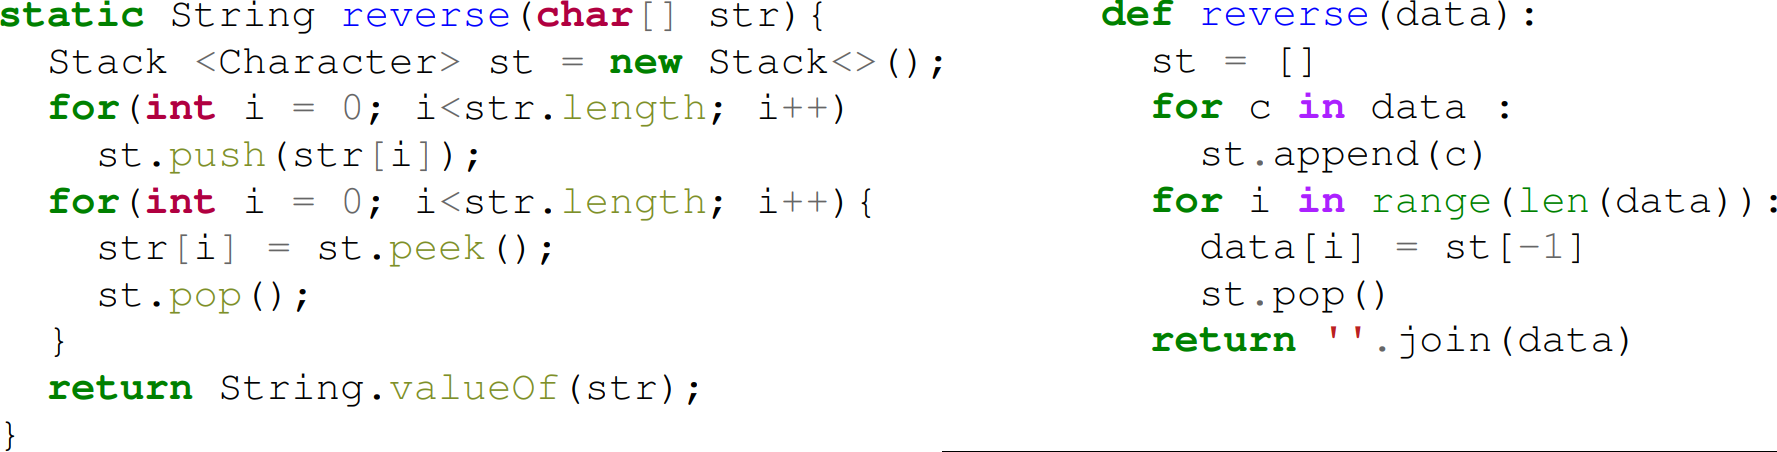
\includegraphics[scale=.34]{./figures/Code_Translation.png}
		\end{center}
		\caption{Unsupervised code translation Java to Python, from \cite{roziere2021leveraging}}
		\label{fig:CodeTranslation}
	\end{figure}

	\end{block}

\end{column}

\separatorcolumn

\begin{column}{\colwidth}

	\begin{block}{Methods}
		%\heading{Overview} % remove?
		%\begin{itemize}
		%	\item Train a Mal2Good model to translate malicious-looking code into benign-looking code
		%	\item Find and replace highly suspicious portions of malware's code with benign-looking code
		%	\item Evaluate the attack's evasion rate against a state of the art malware detector
		%\end{itemize}
		
		%\heading{Overview}
		%\begin{itemize}
		%	\item Identify suspicious sections of code within the malware
		%	\item Translate them into benign-looking format
		%	\item Verify malware functionality remains intact
		%\end{itemize}

		\heading{Identifying Code A Classifier Finds Suspicious}
		\begin{itemize}
			\item Neural networks can detect malware from raw bytes
			\item Explainability algorithms can identify suspicious code
		\end{itemize}
		
		\begin{figure}
			\begin{center}
				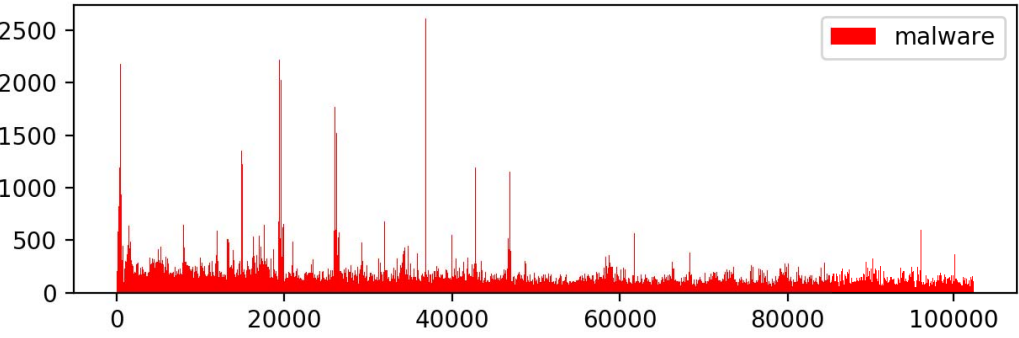
\includegraphics[scale=.5]{./figures/Explainability.png}
			\end{center}
			\caption{Large gradient activations indicate suspicious code, from \cite{coull2019activation}}
			\label{fig:ExplainabilityFileOffset}
		\end{figure}

		\heading{Translating Suspicious Code To Appear Benign}
		\begin{itemize}
			\item mal2good: a fully unsupervised malicious-looking to benign-looking assembly code translation model
			\item Encoder-decoder architecture trained with language modeling, denoising auto encoding, and backtranslation
			\item Use mal2good to replace suspicious portions of code
		\end{itemize}
		
		\begin{figure}
			\begin{center}
				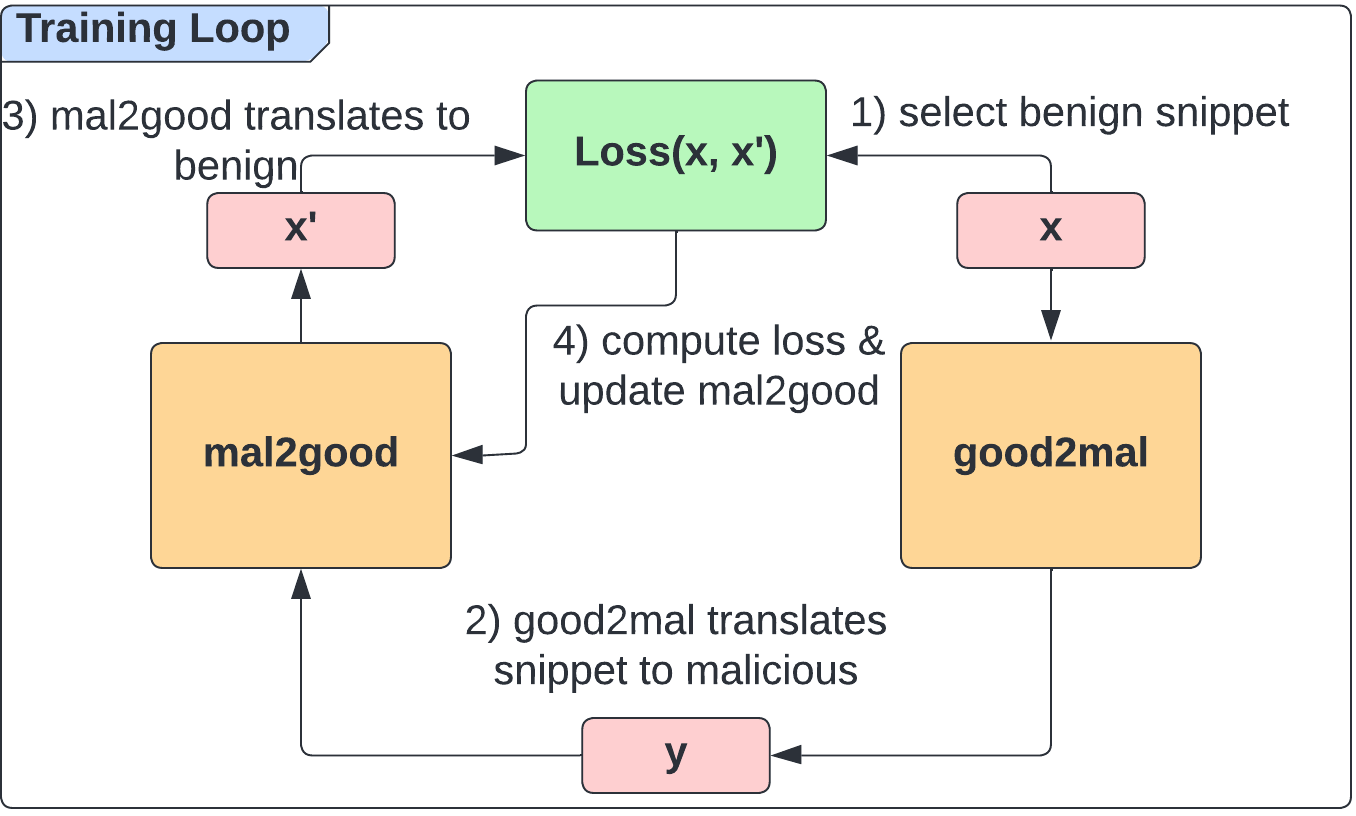
\includegraphics[scale=1.25]{./figures/Backtranslation.png}
			\end{center}
			\caption{Backtranslation simultaneously trains forward and backward translation models (only learning forward model shown)}
			\label{fig:Backtranslation}
		\end{figure}
		
	\end{block}

\end{column}

\separatorcolumn

\begin{column}{\colwidth}

	\begin{block}{Experiment}
		
		%\heading{Research Questions} 
		%\begin{itemize}
		%	\item How well does our attack perform against a raw byte CNN classifier in a white box scenario?
		%	\item How do these adversarial examples air against non-CNN and code-only detectors?
		%	\item Can our attack be combined with other attacks to result in an even more powerful attack?
		%\end{itemize}s
		
		\begin{itemize}
			\item Create adversarial malware and measure evasion rate
			\item Test adversarial examples against additional classifiers
			\item Compare performance against other adversarial attacks
		\end{itemize}
	
		\begin{figure}
			\begin{center}
				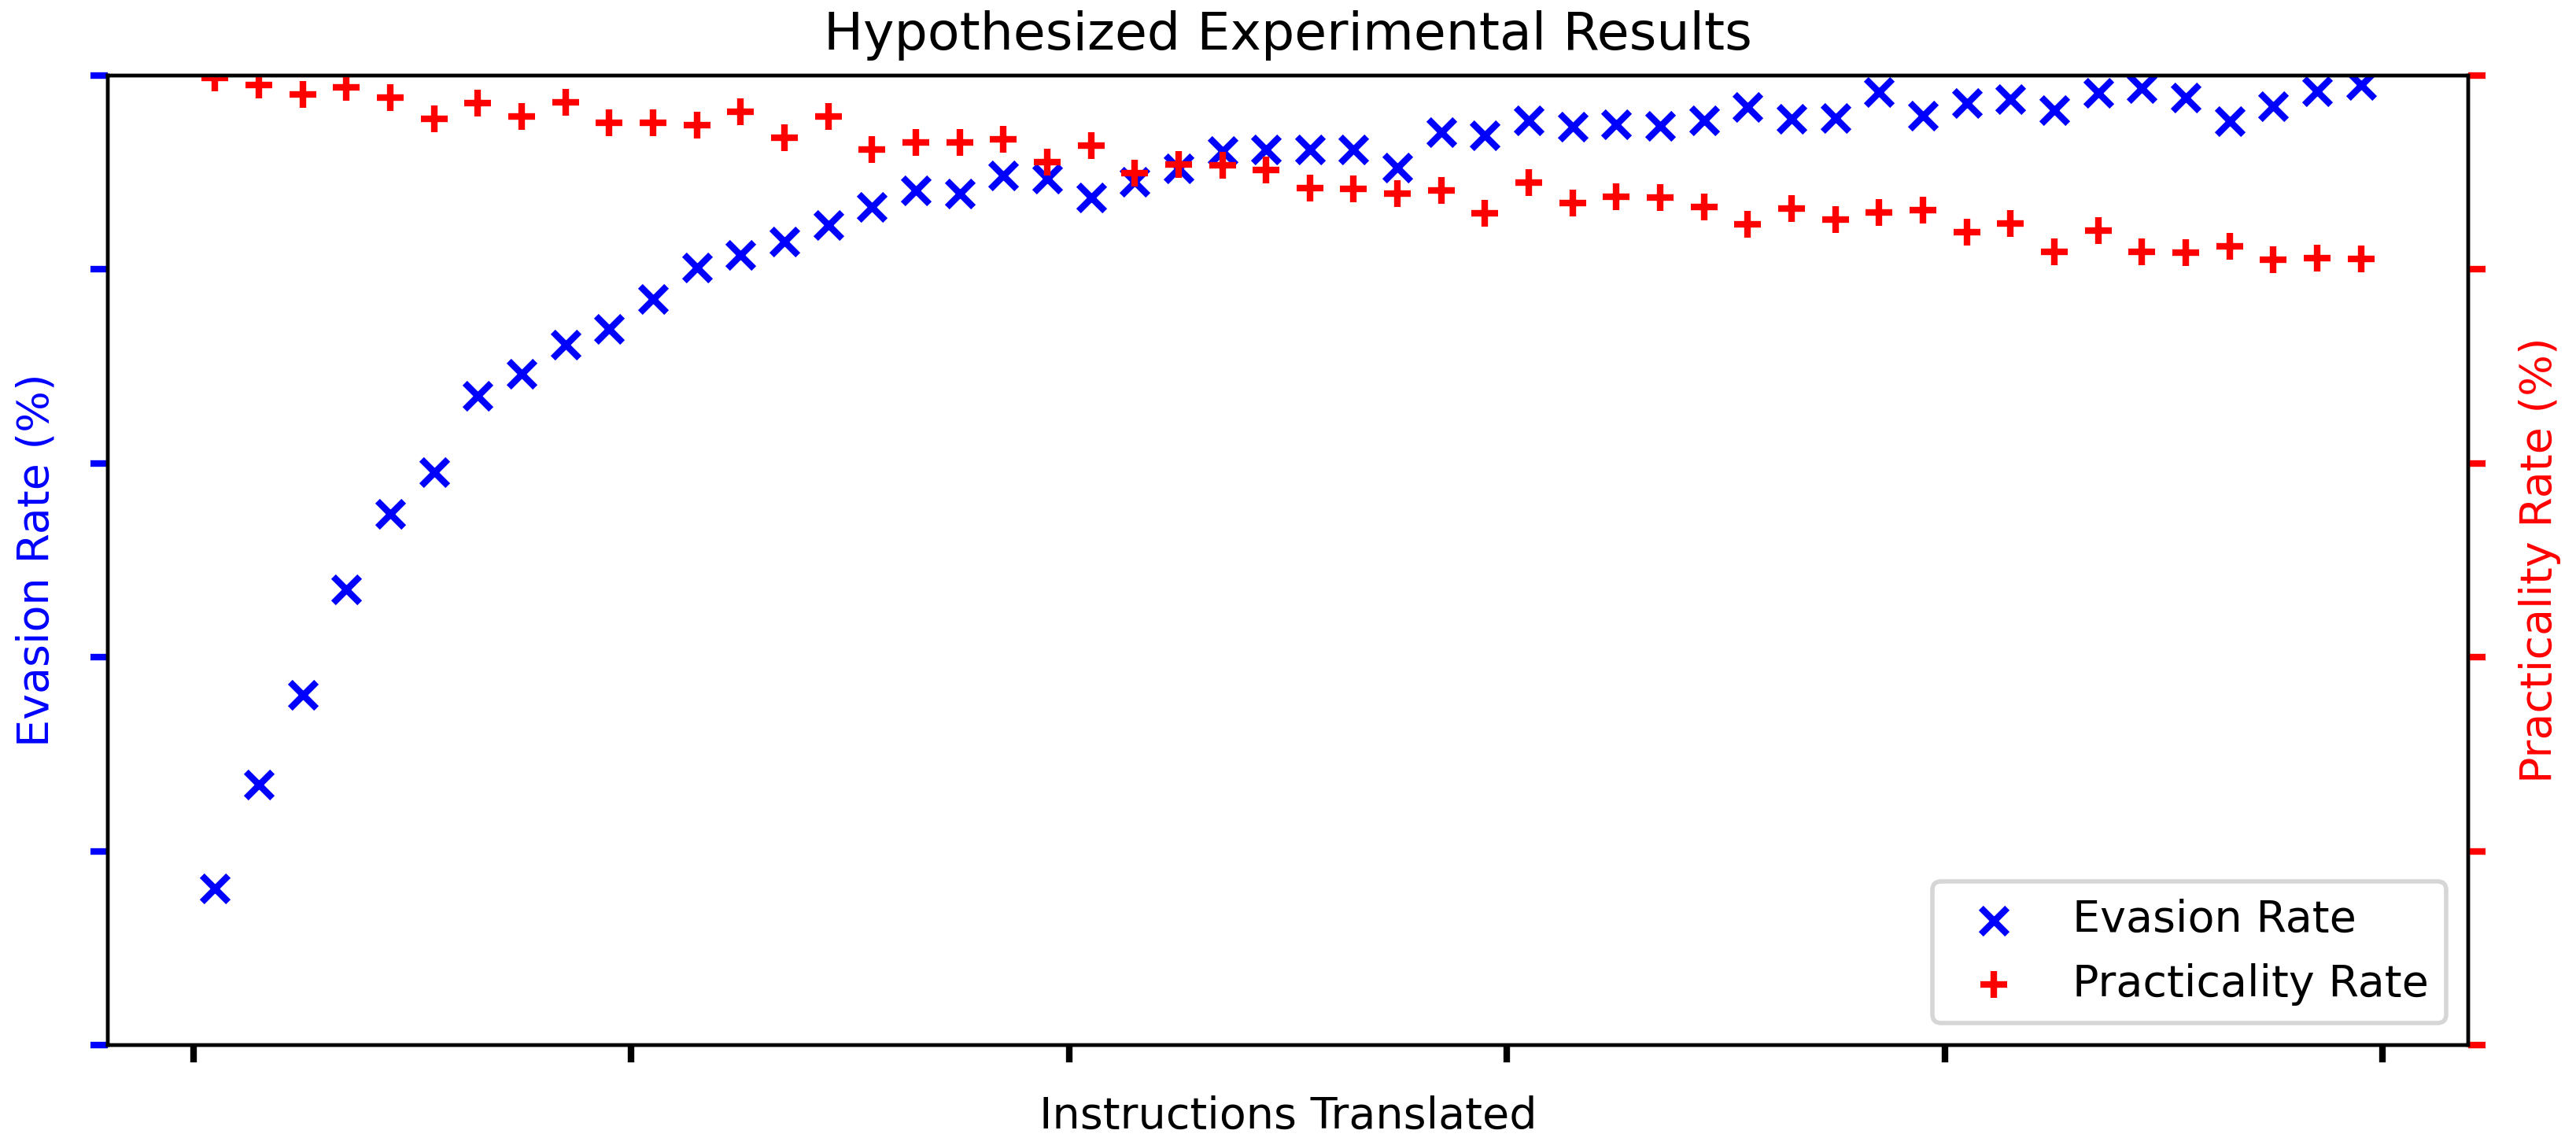
\includegraphics[scale=.95]{./figures/Evasion_Rate.png}
			\end{center}
			\caption{Translating more instructions should increase the evasion rate but decrease the percent of malware that is practical/executes properly (plot is purely speculative, no results have been obtained)}
			\label{fig:EvasionRate}
		\end{figure}
		
	\end{block}
	
	\begin{block}{Challenges}
		
		\begin{itemize}
			\item mal2good must produce semantically correct code
			\item mal2good must produce code that appears benign
			\item mal2good must be trained in an unsupervised manner
			\item Challenging to evaluate mal2good's performance
		\end{itemize}
	
		%\heading{Challenges}
		%\begin{itemize}
		%	\item Mal2Good must be trained in a fully unsupervised setting
	    %	\item Mal2Good must produce code that looks benign to malware classifier
	    %	\item Mal2Good must produce syntactically and semantically correct code
		%\end{itemize}
	
		%\heading{Merits} % remove?
		%\begin{itemize}
		%	\item Novel practical adversarial attack that rewrites malware's executable code
		%	\item Novel concept modeling malware and benignware as distinct languages
		%	\item Novel application of unsupervised NMT to assembly-to-assembly translation
		%\end{itemize}
	
	\end{block}
	
	\begin{block}{References}
	
		%\nocite{*}
		\scriptsize{\bibliographystyle{plain}\bibliography{master}}
	
	\end{block}

\end{column}

\separatorcolumn
\end{columns}
\end{frame}

\end{document}
